\documentclass[a4paper]{article}
\usepackage{vntex}
%\usepackage[enetglish,vinam]{babel}
%\usepackage[utf8]{inputenc}
\usepackage{mathptmx}[ptm]
%\usepackage[utf8]{inputenc}
%\usepackage[francais]{babel}
\usepackage{a4wide,amssymb,epsfig,latexsym,array,hhline,fancyhdr}
\usepackage[normalem]{ulem}
%\usepackage{soul}

\usepackage[makeroom]{cancel}
\usepackage{amsmath}
\usepackage{amsthm}
\usepackage{multicol,longtable,amscd}
\usepackage{diagbox}%Make diagonal lines in tables
\usepackage{booktabs}
\usepackage{alltt}
\usepackage[framemethod=tikz]{mdframed}% For highlighting paragraph backgrounds
\usepackage{caption,subcaption}

\usepackage{lastpage}
\usepackage[lined,boxed,commentsnumbered]{algorithm2e}
\usepackage{enumerate}
\usepackage{color}
\usepackage{graphicx}							% Standard graphics package
\usepackage{array}
\usepackage{tabularx, caption}
\usepackage{multirow}
\usepackage{multicol}
\usepackage{rotating}
\usepackage{graphics}
\usepackage{geometry}
\usepackage{setspace}
\usepackage{epsfig}
\usepackage{tikz}

\usetikzlibrary{arrows,snakes,backgrounds,calc}
\usepackage[unicode]{hyperref}
\hypersetup{urlcolor=blue,linkcolor=black,citecolor=black,colorlinks=true} 
\usepackage{listings}

%\usepackage{pstcol} 								% PSTricks with the standard color package

\usepackage[normalem]{ulem}

\newtheorem{theorem}{{\bf Định lý}}
\newtheorem{property}{{\bf Tính chất}}
\newtheorem{proposition}{{\bf Mệnh đề}}
\newtheorem{corollary}[proposition]{{\bf Hệ quả}}
\newtheorem{lemma}[proposition]{{\bf Bổ đề}}
\theoremstyle{definition}
\newtheorem{exer}{Bài toán}
\addtocontents{toc}{\protect\thispagestyle{empty}}
% Remove page number in contents page. 
\addtocontents{lof}{\protect\thispagestyle{empty}}
% Remove page number in list of figure page. 
\addtocontents{lot}{\protect\thispagestyle{empty}}
% Remove page number in list of table page. 
\def\thesislayout{	% A4: 210 × 297
	\geometry{
		a4paper,
		total={160mm,240mm},  % fix over page
		left=30mm,
		top=22mm,
            right=20mm,
            bottom=20mm,
	}
}
\def\thesisheadlayout{	% A4: 210 × 297
	\geometry{
		a4paper,
		total={160mm,240mm},  % fix over page
		left=30mm,
		top=10mm,
	}
}
\thesislayout
\lstset{
language=R,
basicstyle=\footnotesize\sffamily,
commentstyle=\ttfamily\color{black},
numbers=left,
numberstyle=\ttfamily\color{black}\footnotesize,
stepnumber=1,
numbersep=5pt,
backgroundcolor=\color{white},
showspaces=false,
showstringspaces=false,
showtabs=false,
frame=single,
tabsize=2,
captionpos=b,
breaklines=true,
breakatwhitespace=false,
title=\lstname,
escapeinside={},
keywordstyle={},
morekeywords={}
}
%\usepackage{fancyhdr}
\setlength{\headheight}{40pt}
\pagestyle{fancy}
\fancyhead{} % clear all header fields
\renewcommand{\footruleskip}{1mm}

\fancyhead[L]{
 \begin{tabular}{rl}
    \begin{picture}(25,15)(0,0)
    \put(0,-8){
\includegraphics[width=10mm, height=10mm]{images/hcmut.png}}
    %\put(0,-8){\epsfig{width=10mm,figure=hcmut.eps}}
   \end{picture}&
	%
\includegraphics[width=8mm, height=8mm]{hcmut.png} & %
	\begin{tabular}{l}
		\textbf{  Trường Đại Học Bách Khoa - Đại học Quốc gia TP.HCM }\\
		\textbf{  Khoa Khoa Học \& Kỹ Thuật Máy Tính}
	\end{tabular} 	
 \end{tabular}
}
\fancyhead[R]{
	\begin{tabular}{l}
		\tiny \bf \\
		\tiny \bf 
	\end{tabular}  }
\fancyfoot{} % clear all footer fields
\fancyfoot[L]{\scriptsize  Báo cáo Bài tập lớn Khai phá dữ liệu - HK2 2024 - 2025}
\fancyfoot[R]{\scriptsize  Trang {\thepage}/\pageref{LastPage}}

\renewcommand{\headrulewidth}{0.3pt}
\renewcommand{\footrulewidth}{0.3pt}

%%%
\setcounter{secnumdepth}{4}
\setcounter{tocdepth}{3}
\makeatletter
\newcounter {subsubsubsection}[subsubsection]
\renewcommand\thesubsubsubsection{\thesubsubsection .\@alph\c@subsubsubsection}
\newcommand\subsubsubsection{\@startsection{subsubsubsection}{4}{\z@}%
                                     {-3.25ex\@plus -1ex \@minus -.2ex}%
                                     {1.5ex \@plus .2ex}%
                                     {\normalfont\normalsize\bfseries}}
\newcommand*\l@subsubsubsection{\@dottedtocline{3}{10.0em}{4.1em}}
\newcommand*{\subsubsubsectionmark}[1]{}
\makeatother

\everymath{\color{black}}%make in-line maths symbols blue to read/check easily

\sloppy
\captionsetup[figure]{labelfont={small,bf},textfont={small,it},belowskip=-1pt,aboveskip=-9pt}
%space remove between caption, figure, and text
\captionsetup[table]{labelfont={small,bf},textfont={small,it},belowskip=-1pt,aboveskip=7pt}
\setlength{\floatsep}{5pt plus 2pt minus 2pt}
\setlength{\textfloatsep}{5pt plus 2pt minus 2pt}
\setlength{\intextsep}{10pt plus 2pt minus 2pt}

\thesislayout
\onehalfspacing

\begin{document}

\begin{titlepage}
\begin{tikzpicture}[remember picture, overlay]
  \draw[line width = 4pt] ($(current page.north west) + (0.4in,-0.5in)$) rectangle ($(current page.south east) + (-0.4in,0.5in)$);
  \draw[line width=1.5pt]
    ($ (current page.north west) + (0.45in,-0.55in) $)
    rectangle
    ($ (current page.south east) + (-0.45in,0.55in) $);
\end{tikzpicture}

\begin{center}
\LARGE \textbf{ĐẠI HỌC QUỐC GIA THÀNH PHỐ HỒ CHÍ MINH} \\
\vspace{0.2cm}
\LARGE \textbf{TRƯỜNG ĐẠI HỌC BÁCH KHOA} \\
\vspace{0.2cm}
\LARGE \textbf{KHOA KHOA HỌC VÀ KĨ THUẬT MÁY TÍNH}
\end{center}

\vspace{0.3cm}

\begin{figure}[h!]
\begin{center}

\includegraphics[width=4cm]{images/hcmut.png}
\end{center}
\end{figure}

\begin{center}
\begin{tabular}{c}
\textbf{{\LARGE BÁO CÁO BÀI TẬP LỚN}} \\
\\
\textbf{{\LARGE KHAI PHÁ DỮ LIỆU}} \\[15pt]
\\
\parbox{0.9\textwidth}{%
    \centering
    \textbf{\LARGE PHÂN TÍCH CÁC YẾU TỐ ẢNH HƯỞNG TỚI GIÁ \\[6pt] NÔNG SẢN VÀ XÂY DỰNG MÔ HÌNH DỰ ĐOÁN}
}
\end{tabular}
\end{center}

\vspace{0.5cm}
\begin{table}[h]
\begin{tabular}{rll}
\\
\\
\hspace{3 cm} &   \textbf{\Large GVHD:} {\Large Bùi Tiến Đức}
\\
\\
\\
\hspace{3 cm} &     \textbf{$\;$ $\;$$\;$$\;$$\;$$\;$$\;$$\;$$\;$$\;$$\;$$\;$$\;$$\;$$\;$$\;$$\;$$\;$$\;$$\;$$\;$$\;$$\;$$\;$$\;$$\;$$\;$$\;$$\;$$\;$$\;$$\;$$\;$$\;$ \Large ---o0o---} 
\\
\\
\hspace{3 cm} &   \textbf{\Large SVTH1:  } {\Large Phan Nguyễn Hữu Phước - 2212720}
\\
\\
\hspace{3 cm}&   \textbf{\Large SVTH2:  }  {\Large .....Họ \& Tên...........(MSSV)}
\\
\\
\end{tabular}
\end{table}
\vspace{0.5cm}
\begin{center}
{\Large TP. HỒ CHÍ MINH, THÁNG 4/2025 }
\end{center}
\end{titlepage}
%\thispagestyle{empty}
\newpage
%%%%%%%%%%%%%%%%%INTRO%%%%%%%%%%%%%%%%%%%
\newpage
\tableofcontents
\newpage
\listoffigures
\newpage
\listoftables
\newpage
\setcounter{page}{1}

%%%%%%%%%%%%%%%%%CONTENTS%%%%%%%%%%%%%%%%%%%
\section{Giới thiệu}

\subsection{Bối cảnh nghiên cứu}
\hspace{0.5cm}Ô nhiễm không khí là một trong những vấn đề môi trường nghiêm trọng nhất hiện nay, đặc biệt là tại các khu vực đô thị. Trong đó, Carbon Monoxide (CO) và Carbon Dioxide (CO2) là hai trong số các chất ô nhiễm không khí quan trọng cần được theo dõi và kiểm soát. CO là một khí độc không màu, không mùi, có thể gây nguy hiểm đến sức khỏe con người khi tiếp xúc ở nồng độ cao. CO2, mặc dù ít độc hơn, nhưng là một trong những khí nhà kính chính góp phần vào biến đổi khí hậu toàn cầu.

\subsection{Mục tiêu nghiên cứu}
\hspace{0.5cm}Dự án này tập trung vào việc phát triển các mô hình học máy để dự đoán nồng độ CO và CO2 trong không khí dựa trên bộ dữ liệu Air Quality từ UCI Machine Learning Repository. Cụ thể, các mục tiêu chính bao gồm:

\begin{itemize}
    \item Phân tích và xử lý dữ liệu từ các cảm biến chất lượng không khí
    \item Xây dựng các mô hình dự đoán nồng độ CO và CO2
    \item Đánh giá hiệu suất của các mô hình dự đoán
    \item Phân tích tầm quan trọng của các yếu tố ảnh hưởng đến nồng độ CO và CO2
\end{itemize}

\subsection{Bộ dữ liệu}
\hspace{0.5cm}Bộ dữ liệu Air Quality được thu thập từ một thiết bị đa cảm biến khí được triển khai tại một thành phố ở Ý. Dữ liệu bao gồm:

\begin{itemize}
    \item Thời gian thu thập: Từ tháng 3/2004 đến tháng 2/2005
    \item Số lượng mẫu: 9,358 mẫu
    \item Tần suất: Trung bình theo giờ
    \item Các đặc trưng chính:
    \begin{itemize}
        \item Nồng độ CO (mg/m³)
        \item Nồng độ các hợp chất hữu cơ không chứa metan (µg/m³)
        \item Nồng độ Benzen (µg/m³)
        \item Nồng độ NOx (ppb)
        \item Nồng độ NO2 (µg/m³)
        \item Nhiệt độ (°C)
        \item Độ ẩm tương đối (\%)
        \item Độ ẩm tuyệt đối (g/m³)
    \end{itemize}
\end{itemize}

\subsection{Ý nghĩa thực tiễn}
\hspace{0.5cm}Nghiên cứu này có ý nghĩa quan trọng trong việc:

\begin{itemize}
    \item Cảnh báo sớm về mức độ ô nhiễm không khí
    \item Hỗ trợ các cơ quan quản lý môi trường trong việc ra quyết định
    \item Nâng cao nhận thức cộng đồng về chất lượng không khí
    \item Góp phần vào việc phát triển các hệ thống giám sát chất lượng không khí thông minh
\end{itemize}

\subsection{Cấu trúc báo cáo}
\hspace{0.5cm}Báo cáo được tổ chức thành các phần chính sau:

\begin{itemize}
    \item Phần 1: Giới thiệu tổng quan về đề tài
    \item Phần 2: Cơ sở lý thuyết về học máy và các mô hình dự đoán
    \item Phần 3: Phương pháp nghiên cứu và xử lý dữ liệu
    \item Phần 4: Kết quả thực nghiệm và đánh giá
    \item Phần 5: Kết luận và hướng phát triển
\end{itemize}

\newpage
\section{Tổng quan công việc}

\subsection{Giới thiệu về phương pháp luận}

\hspace{0.5cm}Trong dự án này, chúng tôi áp dụng phương pháp luận CRISP-DM (Cross-Industry Standard Process for Data Mining) để thực hiện quá trình khai thác dữ liệu. Phương pháp này bao gồm 6 giai đoạn chính:

\begin{itemize}
    \item \textbf{Hiểu biết về nghiệp vụ (Business Understanding):} Xác định mục tiêu và yêu cầu của dự án
    \item \textbf{Hiểu biết về dữ liệu (Data Understanding):} Thu thập và phân tích dữ liệu ban đầu
    \item \textbf{Chuẩn bị dữ liệu (Data Preparation):} Tiền xử lý và làm sạch dữ liệu
    \item \textbf{Mô hình hóa (Modeling):} Xây dựng và đánh giá các mô hình
    \item \textbf{Đánh giá (Evaluation):} Đánh giá kết quả và kiểm tra mục tiêu
    \item \textbf{Triển khai (Deployment):} Triển khai và duy trì mô hình
\end{itemize}

\subsection{Phương pháp tiếp cận}

\hspace{0.5cm}Dự án sử dụng phương pháp tiếp cận dựa trên dữ liệu (Data-Driven Approach) để phân tích và dự đoán năng suất cây trồng. Các bước thực hiện bao gồm:

\begin{itemize}
    \item \textbf{Thu thập dữ liệu:}
    \begin{itemize}
        \item Sử dụng các nguồn dữ liệu đa dạng (CSV, Excel)
        \item Tích hợp dữ liệu từ nhiều nguồn khác nhau
        \item Đảm bảo tính nhất quán và độ tin cậy của dữ liệu
    \end{itemize}
    
    \item \textbf{Tiền xử lý dữ liệu:}
    \begin{itemize}
        \item Xử lý dữ liệu thiếu và trùng lặp
        \item Chuẩn hóa và mã hóa dữ liệu
        \item Phát hiện và xử lý ngoại lệ
    \end{itemize}
    
    \item \textbf{Phân tích dữ liệu:}
    \begin{itemize}
        \item Phân tích thống kê mô tả
        \item Phân tích tương quan giữa các biến
        \item Phân tích xu hướng theo thời gian
    \end{itemize}
    
    \item \textbf{Xây dựng mô hình:}
    \begin{itemize}
        \item Lựa chọn các thuật toán phù hợp
        \item Huấn luyện và tối ưu hóa mô hình
        \item Đánh giá hiệu suất mô hình
    \end{itemize}
\end{itemize}

\subsection{Các kỹ thuật sử dụng}

\hspace{0.5cm}Dự án áp dụng các kỹ thuật khai thác dữ liệu sau:

\begin{itemize}
    \item \textbf{Phân tích thống kê:}
    \begin{itemize}
        \item Thống kê mô tả (mean, median, mode, standard deviation)
        \item Phân tích tương quan (correlation analysis)
        \item Kiểm định giả thuyết (hypothesis testing)
    \end{itemize}
    
    \item \textbf{Học máy:}
    \begin{itemize}
        \item Học có giám sát (supervised learning)
        \item Học không giám sát (unsupervised learning)
        \item Học bán giám sát (semi-supervised learning)
    \end{itemize}
    
    \item \textbf{Xử lý dữ liệu:}
    \begin{itemize}
        \item Chuẩn hóa dữ liệu (MinMaxScaler)
        \item Mã hóa one-hot (one-hot encoding)
        \item Xử lý ngoại lệ (outlier detection)
    \end{itemize}
    
    \item \textbf{Trực quan hóa dữ liệu:}
    \begin{itemize}
        \item Biểu đồ phân tán (scatter plots)
        \item Biểu đồ đường (line plots)
        \item Biểu đồ boxplot
        \item Heatmap tương quan
    \end{itemize}
\end{itemize}

\subsection{Đánh giá và kiểm chứng}

\hspace{0.5cm}Quá trình đánh giá và kiểm chứng được thực hiện thông qua:

\begin{itemize}
    \item \textbf{Phân chia dữ liệu:}
    \begin{itemize}
        \item Tập huấn luyện (training set)
        \item Tập kiểm định (validation set)
        \item Tập kiểm tra (test set)
    \end{itemize}
    
    \item \textbf{Đánh giá mô hình:}
    \begin{itemize}
        \item Độ chính xác (accuracy)
        \item Precision và Recall
        \item F1-score
        \item RMSE (Root Mean Square Error)
        \item MAE (Mean Absolute Error)
    \end{itemize}
    
    \item \textbf{Kiểm chứng chéo:}
    \begin{itemize}
        \item K-fold cross validation
        \item Leave-one-out cross validation
    \end{itemize}
\end{itemize}

\subsection{Tính mới và đóng góp}

\hspace{0.5cm}Dự án mang lại các đóng góp mới trong lĩnh vực khai thác dữ liệu nông nghiệp:

\begin{itemize}
    \item \textbf{Phương pháp tích hợp dữ liệu:}
    \begin{itemize}
        \item Tích hợp dữ liệu từ nhiều nguồn khác nhau
        \item Xử lý tự động các vấn đề về dữ liệu
        \item Đảm bảo tính nhất quán của dữ liệu
    \end{itemize}
    
    \item \textbf{Cải tiến trong xử lý dữ liệu:}
    \begin{itemize}
        \item Tự động phát hiện và xử lý ngoại lệ
        \item Chuẩn hóa dữ liệu thông minh
        \item Mã hóa dữ liệu phân loại hiệu quả
    \end{itemize}
    
    \item \textbf{Ứng dụng thực tế:}
    \begin{itemize}
        \item Dự đoán năng suất cây trồng
        \item Phân tích ảnh hưởng của các yếu tố môi trường
        \item Hỗ trợ ra quyết định trong nông nghiệp
    \end{itemize}
\end{itemize}

\subsection*{Tóm Tắt}
Phương pháp luận của dự án kết hợp các kỹ thuật khai thác dữ liệu hiện đại với quy trình CRISP-DM, tập trung vào việc xử lý và phân tích dữ liệu nông nghiệp. Các kỹ thuật được áp dụng bao gồm phân tích thống kê, học máy, và trực quan hóa dữ liệu, nhằm đạt được kết quả chính xác và có ý nghĩa thực tiễn. 
\newpage
\section{Cơ sở lý thuyết}
\subsection{ Các yếu tố ảnh hưởng đến giá nông sản}

Giá nông sản là một biến số nhạy cảm, chịu ảnh hưởng bởi nhiều yếu tố phức tạp từ cả phía cung và cầu. Việc hiểu rõ các yếu tố này không chỉ giúp phân tích chính xác mà còn là nền tảng để xây dựng các mô hình dự đoán hiệu quả. Một số yếu tố chủ yếu bao gồm:

\begin{itemize}
    \item \textbf{Thời tiết và khí hậu:} Nhiệt độ, lượng mưa, hạn hán, lũ lụt và các hiện tượng thời tiết cực đoan ảnh hưởng trực tiếp đến năng suất và chất lượng cây trồng.
    
    \item \textbf{Dịch bệnh và sâu bệnh:} Sự bùng phát của sâu bệnh làm giảm sản lượng và chất lượng nông sản, từ đó đẩy giá thành lên cao.

    \item \textbf{Chi phí đầu vào:} Bao gồm giá giống cây trồng, phân bón, nhân công và đặc biệt là \textbf{thuốc trừ sâu}. Việc sử dụng thuốc trừ sâu không chỉ ảnh hưởng đến chi phí sản xuất mà còn tác động đến chất lượng sản phẩm, từ đó ảnh hưởng đến giá cả.

    \item \textbf{Chính sách nhà nước:} Các chính sách về thuế, trợ cấp, khuyến khích sản xuất hoặc hạn chế xuất khẩu cũng ảnh hưởng lớn đến giá nông sản.

    \item \textbf{Quan hệ cung - cầu thị trường:} Khi sản lượng vượt cầu, giá sẽ giảm; ngược lại khi nguồn cung hạn chế, giá có xu hướng tăng.

    \item \textbf{Tác động từ thị trường quốc tế:} Biến động giá cả toàn cầu, tỉ giá hối đoái và tình hình xuất nhập khẩu đều tác động đến giá nông sản trong nước.
\end{itemize}

Những yếu tố này thường có mối quan hệ phức tạp và phi tuyến tính với giá nông sản, khiến cho việc phân tích và dự đoán trở thành một bài toán đầy thách thức nhưng cũng rất cần thiết và có tính ứng dụng cao trong thực tiễn.


\subsection{ Tổng quan về học máy và phân lớp dữ liệu}

Học máy (\textit{Machine Learning}) là một nhánh của trí tuệ nhân tạo (AI), cho phép máy tính học từ dữ liệu và cải thiện hiệu suất dự đoán mà không cần lập trình một cách cụ thể. Trong bối cảnh dự đoán giá nông sản, học máy đóng vai trò quan trọng trong việc xây dựng các mô hình có khả năng khai thác các mối quan hệ phức tạp giữa nhiều yếu tố ảnh hưởng khác nhau.

Học máy được chia thành nhiều loại, trong đó phổ biến nhất là:
\begin{itemize}
    \item \textbf{Học có giám sát (Supervised Learning):} Mô hình được huấn luyện trên tập dữ liệu có nhãn, tức là mỗi mẫu dữ liệu đều đi kèm với kết quả đầu ra mong muốn. Đây là phương pháp chính được sử dụng trong bài toán dự đoán giá nông sản.
    
    \item \textbf{Học không giám sát (Unsupervised Learning):} Tập trung vào việc tìm kiếm cấu trúc ẩn trong dữ liệu không có nhãn (ví dụ: phân cụm).
    
    \item \textbf{Học tăng cường (Reinforcement Learning):} Mô hình học thông qua tương tác với môi trường và tối ưu hóa phần thưởng.
\end{itemize}

Trong khuôn khổ đồ án này, bài toán chính được xác định là một bài toán \textbf{hồi quy}, trong đó đầu ra cần dự đoán là một giá trị liên tục (giá nông sản). Tuy nhiên, cũng có thể tiếp cận dưới dạng \textbf{phân lớp} nếu ta chia giá thành các mức giá cụ thể như “thấp”, “trung bình” và “cao”.

Các thuật toán học máy thường được sử dụng trong phân tích và dự đoán dữ liệu gồm có: hồi quy tuyến tính, cây quyết định, xác suất Bayes (Naive Bayes), mạng nơ-ron nhân tạo và K-nearest neighbors (KNN). Mỗi thuật toán có đặc điểm riêng phù hợp với từng kiểu dữ liệu và yêu cầu dự đoán khác nhau, sẽ được trình bày cụ thể ở phần tiếp theo.


\subsection{ Các thuật toán học máy}

Trong quá trình xây dựng mô hình dự đoán giá nông sản, việc lựa chọn thuật toán phù hợp là yếu tố then chốt để đảm bảo độ chính xác và khả năng tổng quát hóa của mô hình. Dưới đây là các thuật toán phổ biến được sử dụng trong bài toán dự đoán giá trị liên tục hoặc phân lớp giá trị.

\subsubsection{ Hồi quy tuyến tính (Linear Regression)}

Hồi quy tuyến tính là một trong những mô hình cơ bản nhất trong học máy, được sử dụng rộng rãi trong các bài toán dự đoán. Mục tiêu của hồi quy tuyến tính là tìm ra một hàm tuyến tính \( y = w_0 + w_1x_1 + w_2x_2 + \ldots + w_nx_n \) sao cho sai số giữa giá trị dự đoán và giá trị thực tế là nhỏ nhất.

\begin{itemize}
    \item \textbf{Ưu điểm:} Dễ hiểu, dễ triển khai, thời gian huấn luyện nhanh.
    \item \textbf{Nhược điểm:} Chỉ phù hợp với các mối quan hệ tuyến tính giữa các biến; độ chính xác không cao khi dữ liệu có quan hệ phi tuyến.
\end{itemize}

\subsubsection{ Cây quyết định (Decision Tree)}

Cây quyết định là mô hình dựa trên cấu trúc cây phân nhánh, trong đó mỗi nút là một điều kiện phân chia dữ liệu dựa trên giá trị của một thuộc tính, và các nhánh dẫn đến các quyết định hoặc dự đoán.

\begin{itemize}
    \item \textbf{Ưu điểm:} Dễ giải thích, không cần chuẩn hóa dữ liệu, xử lý tốt dữ liệu hỗn hợp.
    \item \textbf{Nhược điểm:} Dễ bị overfitting nếu cây quá sâu, kém ổn định với dữ liệu nhiễu.
\end{itemize}

\subsubsection{ Naive Bayes (Xác suất Bayes ngây thơ)}

Naive Bayes là mô hình phân loại dựa trên định lý Bayes, với giả định rằng các đặc trưng là độc lập với nhau (giả định “ngây thơ”). Mô hình này được tính dựa trên công thức:

\[
P(C|X) = \frac{P(X|C) \cdot P(C)}{P(X)}
\]

Trong đó:
\begin{itemize}
    \item \( P(C|X) \): xác suất một mẫu \( X \) thuộc về lớp \( C \)
    \item \( P(X|C) \): xác suất quan sát thấy \( X \) nếu biết nó thuộc lớp \( C \)
    \item \( P(C) \): xác suất xảy ra của lớp \( C \)
    \item \( P(X) \): xác suất xảy ra của dữ liệu \( X \)
\end{itemize}

\begin{itemize}
    \item \textbf{Ưu điểm:} Tốc độ xử lý nhanh, hiệu quả với dữ liệu lớn, dễ cài đặt.
    \item \textbf{Nhược điểm:} Giả định độc lập giữa các đặc trưng thường không đúng trong thực tế.
\end{itemize}

\subsubsection{ Mạng nơ-ron nhân tạo (Artificial Neural Network - ANN)}

Mạng nơ-ron nhân tạo là mô hình học sâu được lấy cảm hứng từ cách hoạt động của bộ não con người. Một mạng nơ-ron bao gồm các lớp (layer) gồm nhiều “nơ-ron” (neuron), được kết nối với nhau thông qua các trọng số. Dữ liệu đầu vào được truyền qua từng lớp (input, hidden, output), trải qua các hàm kích hoạt và được huấn luyện bằng cách cập nhật trọng số để giảm sai số dự đoán.

\begin{itemize}
    \item \textbf{Ưu điểm:} Khả năng mô hình hóa các mối quan hệ phi tuyến phức tạp, phù hợp với dữ liệu lớn và nhiều chiều.
    \item \textbf{Nhược điểm:} Cần nhiều tài nguyên tính toán, dễ overfitting nếu không điều chỉnh tốt; khó giải thích kết quả so với các mô hình truyền thống.
\end{itemize}

Trong bài toán dự đoán giá nông sản, ANN đặc biệt hiệu quả khi có dữ liệu lớn, với nhiều đặc trưng đầu vào như thời tiết, phân bón, thuốc trừ sâu, v.v.

\subsubsection{ K-Nearest Neighbors (KNN)}

KNN là thuật toán đơn giản nhưng mạnh mẽ, dựa trên nguyên lý “gần mực thì đen, gần đèn thì sáng”. Khi cần dự đoán một điểm mới, KNN sẽ tìm \( k \) điểm dữ liệu gần nhất trong không gian đặc trưng, sau đó lấy trung bình (đối với bài toán hồi quy) hoặc đa số (đối với phân lớp) làm kết quả.

\begin{itemize}
    \item \textbf{Ưu điểm:} Dễ triển khai, không giả định phân phối dữ liệu.
    \item \textbf{Nhược điểm:} Tốc độ chậm khi dữ liệu lớn, nhạy cảm với nhiễu và khoảng cách.
\end{itemize}

Việc lựa chọn giá trị \( k \) phù hợp là yếu tố then chốt quyết định hiệu quả của mô hình KNN.

\newpage
\section{Preprocessing Data (Tiền xử lý dữ liệu)}

\subsection{Giới thiệu chung về vai trò của tiền xử lý dữ liệu trong khai thác dữ liệu}

\hspace{0.5cm}Trong dự án này, tiền xử lý dữ liệu đóng vai trò quan trọng trong việc chuẩn bị dữ liệu về chất lượng không khí cho mô hình học máy. Dữ liệu thô (\textit{raw data}) chứa thông tin về các chỉ số ô nhiễm không khí, nhiệt độ, độ ẩm và thời gian, cần được xử lý để đảm bảo tính chính xác và hiệu quả của mô hình dự đoán.

\begin{figure}[htbp]
    \centering
    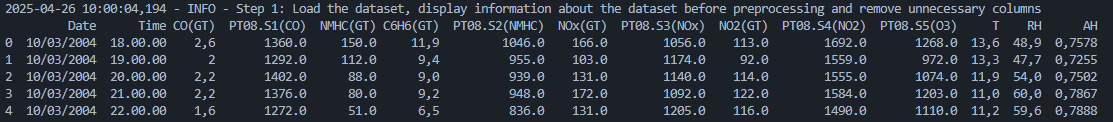
\includegraphics[width=0.9\textwidth]{images/raw_data_preview.png}
    \vspace{0.5cm}
    \caption{Hiển thị dữ liệu gốc trước khi tiền xử lý}
    \label{fig:raw_data_preview}
\end{figure}

\begin{figure}[htbp]
    \centering
    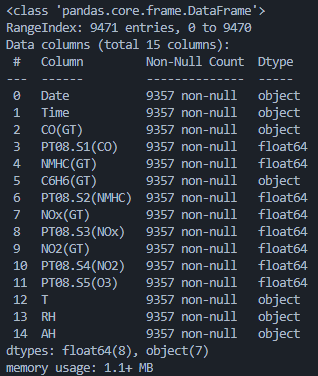
\includegraphics[width=0.45\textwidth]{images/raw_data_statistics.png}
    \vspace{0.5cm}
    \caption{Thống kê mô tả dữ liệu gốc}
    \label{fig:raw_data_statistics}
\end{figure}

\subsection{Ý nghĩa của các đặc trưng}

\begin{description}
    \item[CO(GT)]: Nồng độ Carbon Monoxide trong không khí, được tính toán là trung bình theo giờ (hourly averaged). Dữ liệu này được thu thập từ một máy phân tích tham chiếu (reference analyzer), có độ chính xác cao. Nồng độ CO được đo bằng mg/m³ (miligram trên mét khối). Carbon monoxide (CO) là một khí độc, không mùi và không màu, có thể gây nguy hiểm nếu nồng độ trong không khí quá cao. Khi nồng độ CO vượt quá mức an toàn, nó có thể gây ra các triệu chứng như chóng mặt, đau đầu, và thậm chí là ngộ độc, nguy hiểm đến tính mạng nếu nồng độ quá cao.

    \item[PT08.S1(CO)]: Phản hồi cảm biến theo giờ (hourly averaged sensor response) của một cảm biến được thiết kế để đo nồng độ khí carbon monoxide (CO). Dữ liệu này là giá trị đo được từ một cảm biến cụ thể (có thể là cảm biến điện hóa hoặc cảm biến quang học) được sử dụng để đo nồng độ CO. Cảm biến này không đo trực tiếp nồng độ CO bằng đơn vị mg/m³ hoặc ppm, mà thay vào đó là đo phản hồi của cảm biến (có thể là tín hiệu điện hay tín hiệu quang học).

    \item[NMHC(GT)]: Nồng độ trung bình theo giờ của các hợp chất hữu cơ không bão hòa (Non-Methane Hydrocarbons - NMHC) trong không khí. Dữ liệu này được thu thập từ một máy phân tích tham chiếu (reference analyzer), và giá trị trong cột này là nồng độ của các hợp chất này, đo bằng microgram mỗi mét khối (µg/m³). NMHC là một nhóm các hợp chất hữu cơ dễ bay hơi (VOCs) không chứa metan. Những hợp chất này thường xuất hiện trong khí thải từ các nguồn như giao thông, công nghiệp, hoặc từ các sản phẩm tiêu dùng như sơn và dung môi.

    \item[C6H6(GT)]: Nồng độ trung bình theo giờ của Benzen (C6H6) trong không khí, đo bằng microgram mỗi mét khối (µg/m³). Benzen là một hợp chất rất nguy hiểm nếu tiếp xúc lâu dài hoặc với nồng độ cao. Nó có thể gây ra các vấn đề nghiêm trọng về sức khỏe, bao gồm các bệnh về máu, ung thư và các vấn đề liên quan đến hệ thần kinh.

    \item[PT08.S2(NMHC)]: Phản hồi cảm biến theo giờ của một cảm biến được thiết kế để đo nồng độ các hợp chất hữu cơ không bão hòa (Non-Methane Hydrocarbons - NMHC) trong không khí. Dữ liệu này không đo nồng độ NMHC trực tiếp bằng các đơn vị như µg/m³ hay ppm, mà là giá trị phản hồi của cảm biến.

    \item[NOx(GT)]: Nồng độ trung bình theo giờ của Nitrogen Oxides (NOx) trong không khí, được đo bằng một máy phân tích tham chiếu. Đơn vị đo trong cột này là ppb (parts per billion). NOx là một nhóm các hợp chất bao gồm Nitrogen Dioxide (NO2) và Nitric Oxide (NO), có thể gây ảnh hưởng đến sức khỏe con người và môi trường.

    \item[PT08.S3(NOx)]: Phản hồi cảm biến theo giờ của một cảm biến được thiết kế để đo nồng độ Nitrogen Oxides (NOx) trong không khí. Dữ liệu này là phản hồi của cảm biến, tính trung bình trong suốt một giờ.

    \item[NO2(GT)]: Nồng độ trung bình theo giờ của Nitrogen Dioxide (NO2) trong không khí, được đo bằng một máy phân tích tham chiếu. Đơn vị đo của cột này là microgram per cubic meter (µg/m³). NO2 là một chất ô nhiễm quan trọng trong không khí, có thể gây ra các vấn đề sức khỏe nghiêm trọng.

    \item[PT08.S4(NO2)]: Phản hồi cảm biến theo giờ của một cảm biến được thiết kế để đo nồng độ Nitrogen Dioxide (NO2) trong không khí. Dữ liệu này là phản hồi cảm biến, tính trung bình trong suốt một giờ.

    \item[PT08.S5(O3)]: Phản hồi cảm biến theo giờ của một cảm biến được thiết kế để đo nồng độ Ozone (O3) trong không khí. Dữ liệu này là phản hồi của cảm biến, được tính trung bình trong suốt một giờ.

    \item[T]: Nhiệt độ (Temperature) trong không khí, được đo bằng đơn vị độ Celsius (°C). Nhiệt độ đóng vai trò quan trọng trong việc xác định điều kiện môi trường và ảnh hưởng đến sự phân tán và pha loãng các chất ô nhiễm.

    \item[RH]: Độ ẩm tương đối (Relative Humidity), được đo bằng đơn vị % (phần trăm). Đây là tỷ lệ giữa lượng hơi nước hiện có trong không khí và lượng hơi nước tối đa mà không khí có thể chứa tại một nhiệt độ nhất định. Độ ẩm tương đối ảnh hưởng lớn đến chất lượng không khí và các phản ứng hóa học trong khí quyển.

    \item[AH]: Độ ẩm tuyệt đối (Absolute Humidity), được đo bằng đơn vị g/m³ (gram trên mét khối). Đây là lượng hơi nước có trong không khí, không phụ thuộc vào nhiệt độ. Độ ẩm tuyệt đối là một chỉ số quan trọng để hiểu rõ hơn về sự thay đổi của lượng hơi nước trong không khí và ảnh hưởng của nó đến chất lượng không khí.

    \item[Date\_Time]: Thời gian đo đạc
    \item[Year, Month, Day, Hour]: Các đặc trưng thời gian
\end{description}

\subsection{Quá trình tiền xử lý dữ liệu}

\subsubsection{Bước 1: Xử lý các cột không cần thiết}
\hspace{0.5cm}Đầu tiên, nhóm loại bỏ các cột không cần thiết như "Unnamed: 15" và "Unnamed: 16" để làm sạch dữ liệu.

\subsubsection{Bước 2: Xử lý giá trị thiếu}
\hspace{0.5cm}Đối với các cột số học, giá trị thiếu được thay thế bằng giá trị trung bình của cột đó. Đối với các cột dạng chuỗi, giá trị thiếu được thay thế bằng giá trị xuất hiện thường xuyên nhất.

\subsubsection{Bước 3: Chuyển đổi kiểu dữ liệu}
\hspace{0.5cm}Các cột dữ liệu được chuyển đổi sang kiểu dữ liệu phù hợp:
\begin{itemize}
    \item Cột "Date" được chuyển đổi từ định dạng DD/MM/YYYY sang datetime
    \item Cột "Time" được chuyển đổi từ định dạng HH.MM.SS sang time
    \item Các cột số học được chuẩn hóa bằng cách thay thế dấu phẩy bằng dấu chấm
    \item Cột CO(GT) có giá trị -200 được thay thế bằng giá trị trung bình
\end{itemize}

\subsubsection{Bước 4: Xử lý ngoại lệ (outliers)}
\hspace{0.5cm}Nhóm sử dụng phương pháp Z-score để xác định và xử lý các giá trị ngoại lệ:
\begin{itemize}
    \item Tính toán Z-score cho mỗi cột số học
    \item Xác định ngưỡng là 3 độ lệch chuẩn
    \item Thay thế các giá trị ngoại lệ bằng giá trị trung bình của cột
    \item Đặc biệt xử lý cột NMHC(GT) để đảm bảo không có giá trị âm
\end{itemize}

\begin{figure}[htbp]
    \centering
    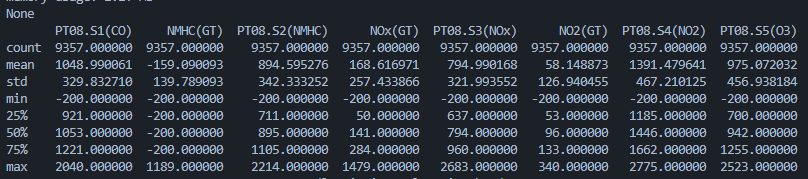
\includegraphics[width=0.9\textwidth]{images/data_distribution_comparison.png}
    \vspace{0.5cm}
    \caption{So sánh phân phối dữ liệu trước và sau khi xử lý ngoại lệ}
    \label{fig:data_distribution}
\end{figure}

\subsubsection{Bước 5: Tạo đặc trưng mới}
\hspace{0.5cm}Nhóm tạo các đặc trưng mới từ dữ liệu hiện có:
\begin{itemize}
    \item Kết hợp cột "Date" và "Time" thành cột "Date\_Time"
    \item Trích xuất thông tin năm, tháng, ngày và giờ từ cột "Date\_Time"
    \item Tạo các đặc trưng tương tác như Temp\_Humidity, NOx\_NO2
    \item Thêm các đặc trưng thống kê như rolling mean và rolling std
\end{itemize}

\subsection{Kết quả tiền xử lý dữ liệu}

\subsubsection{Thông tin tổng quan về dữ liệu}
\hspace{0.5cm}Sau khi tiền xử lý, bộ dữ liệu có các đặc điểm sau:
\begin{itemize}
    \item Số lượng mẫu: 9,471
    \item Số lượng đặc trưng: 18
    \item Các kiểu dữ liệu:
    \begin{itemize}
        \item float64: 13 cột
        \item datetime64[ns]: 1 cột
        \item int32: 4 cột
    \end{itemize}
\end{itemize}

\begin{figure}[htbp]
    \centering
    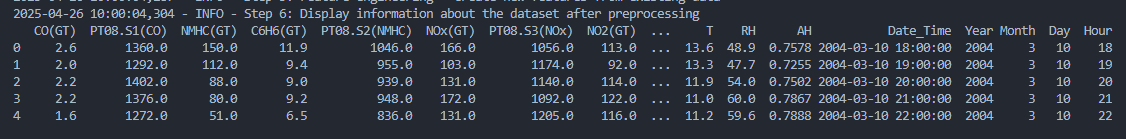
\includegraphics[width=0.9\textwidth]{images/processed_data_preview.png}
    \vspace{0.5cm}
    \caption{Hiển thị dữ liệu sau khi tiền xử lý}
    \label{fig:processed_data_preview}
\end{figure}

\subsubsection{Thống kê mô tả}
\hspace{0.5cm}Các thống kê chính của dữ liệu sau tiền xử lý:
\begin{itemize}
    \item CO(GT): Giá trị trung bình 0.77, dao động từ -5.12 đến 11.90
    \item PT08.S1(CO): Giá trị trung bình 1097.15, dao động từ 647 đến 2008
    \item NMHC(GT): Giá trị trung bình 213.58, dao động từ 29 đến 405
    \item C6H6(GT): Giá trị trung bình 10.06, dao động từ 0.10 đến 63.70
\end{itemize}

\begin{figure}[htbp]
    \centering
    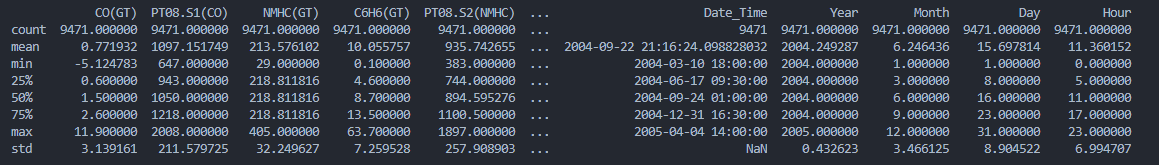
\includegraphics[width=0.45\textwidth]{images/processed_data_statistics.png}
    \vspace{0.5cm}
    \caption{Thống kê mô tả dữ liệu sau tiền xử lý}
    \label{fig:processed_data_statistics}
\end{figure}

\subsection{Kết luận}
\hspace{0.5cm}Quá trình tiền xử lý dữ liệu đã giúp chuẩn bị bộ dữ liệu chất lượng không khí cho việc xây dựng mô hình học máy. Các bước xử lý đã giải quyết các vấn đề về giá trị thiếu, ngoại lệ và tạo thêm các đặc trưng có ý nghĩa. Kết quả cho thấy dữ liệu đã được chuẩn hóa và sẵn sàng cho việc huấn luyện mô hình.
\newpage
\section{Mô hình Random Forest}

\subsection{Giới thiệu}
Mô hình Random Forest đã được triển khai để dự đoán nồng độ CO (Carbon Monoxide) trong không khí dựa trên các thông số môi trường khác nhau. Đây là một mô hình học máy mạnh mẽ thuộc họ Ensemble Learning, kết hợp nhiều cây quyết định để tạo ra dự đoán chính xác hơn.

\subsection{Quy trình Xử lý Dữ liệu}

\subsubsection{Tiền xử lý dữ liệu}
\begin{itemize}
    \item Loại bỏ các cột không cần thiết
    \item Xử lý giá trị thiếu:
    \begin{itemize}
        \item Thay thế giá trị thiếu trong cột số bằng giá trị trung bình
        \item Thay thế giá trị thiếu trong cột phân loại bằng giá trị xuất hiện nhiều nhất
    \end{itemize}
    \item Chuyển đổi kiểu dữ liệu:
    \begin{itemize}
        \item Chuyển cột Date từ định dạng DD/MM/YYYY sang datetime
        \item Chuyển cột Time từ định dạng HH.MM.SS sang time
        \item Xử lý các giá trị âm trong cột CO(GT) bằng cách thay thế bằng giá trị trung bình
    \end{itemize}
\end{itemize}

\subsubsection{Kỹ thuật Feature Engineering}
Mô hình đã tạo ra các đặc trưng mới để cải thiện hiệu suất:
\begin{itemize}
    \item Tương tác giữa các đặc trưng:
    \begin{itemize}
        \item \texttt{NOx\_Temp}: Tương tác giữa NOx và nhiệt độ
        \item \texttt{NO2\_Humidity}: Tương tác giữa NO2 và độ ẩm
        \item \texttt{Temp\_Humidity}: Tương tác giữa nhiệt độ và độ ẩm
        \item \texttt{NOx\_NO2}: Tương tác giữa NOx và NO2
    \end{itemize}
    \item Đặc trưng đa thức:
    \begin{itemize}
        \item \texttt{NOx\_squared}: Bình phương NOx
        \item \texttt{NO2\_squared}: Bình phương NO2
        \item \texttt{Temp\_squared}: Bình phương nhiệt độ
        \item \texttt{RH\_squared}: Bình phương độ ẩm
    \end{itemize}
    \item Đặc trưng thời gian:
    \begin{itemize}
        \item \texttt{Hour\_sin} và \texttt{Hour\_cos}: Biểu diễn chu kỳ giờ
        \item \texttt{Month\_sin} và \texttt{Month\_cos}: Biểu diễn chu kỳ tháng
    \end{itemize}
    \item Tỷ lệ giữa các đặc trưng:
    \begin{itemize}
        \item \texttt{NOx\_NO2\_ratio}: Tỷ lệ giữa NOx và NO2
    \end{itemize}
    \item Đặc trưng cửa sổ trượt:
    \begin{itemize}
        \item Tính trung bình và độ lệch chuẩn trong cửa sổ 3 điểm cho các đặc trưng quan trọng:
        \begin{itemize}
            \item Nhiệt độ (T)
            \item Độ ẩm tương đối (RH)
            \item NOx
            \item NO2
            \item CO
        \end{itemize}
    \end{itemize}
\end{itemize}

\subsection{Kiến trúc Mô hình Random Forest}

\subsubsection{Tham số Mô hình}
Mô hình được triển khai với các tham số tối ưu:
\begin{itemize}
    \item \texttt{n\_estimators}: 200 cây quyết định
    \item \texttt{max\_depth}: 10 (giới hạn độ sâu tối đa)
    \item \texttt{min\_samples\_split}: 4 mẫu tối thiểu để tách nút
    \item \texttt{random\_state}: 42 để đảm bảo khả năng tái lập kết quả
\end{itemize}

\subsubsection{Quy trình Huấn luyện}
\begin{enumerate}
    \item Chuẩn hóa dữ liệu sử dụng StandardScaler
    \item Chia dữ liệu thành tập huấn luyện (80\%) và tập kiểm tra (20\%)
    \item Huấn luyện mô hình trên tập huấn luyện
    \item Đánh giá hiệu suất trên tập kiểm tra
\end{enumerate}

\subsection{Kết quả và Đánh giá}

\subsubsection{Các chỉ số Đánh giá}
Mô hình đạt được kết quả ấn tượng với các chỉ số sau:
\begin{itemize}
    \item Mean Squared Error (MSE): 0.0002
    \item Root Mean Squared Error (RMSE): 0.0136
    \item Mean Absolute Error (MAE): 0.0053
    \item R-squared (R²): 0.9992
\end{itemize}

\subsubsection{Trực quan hóa Kết quả}
Các biểu đồ được tạo ra để phân tích kết quả:
\begin{itemize}
    \item Biểu đồ so sánh giá trị thực tế và dự đoán:
    \begin{figure}[h]
        \centering
        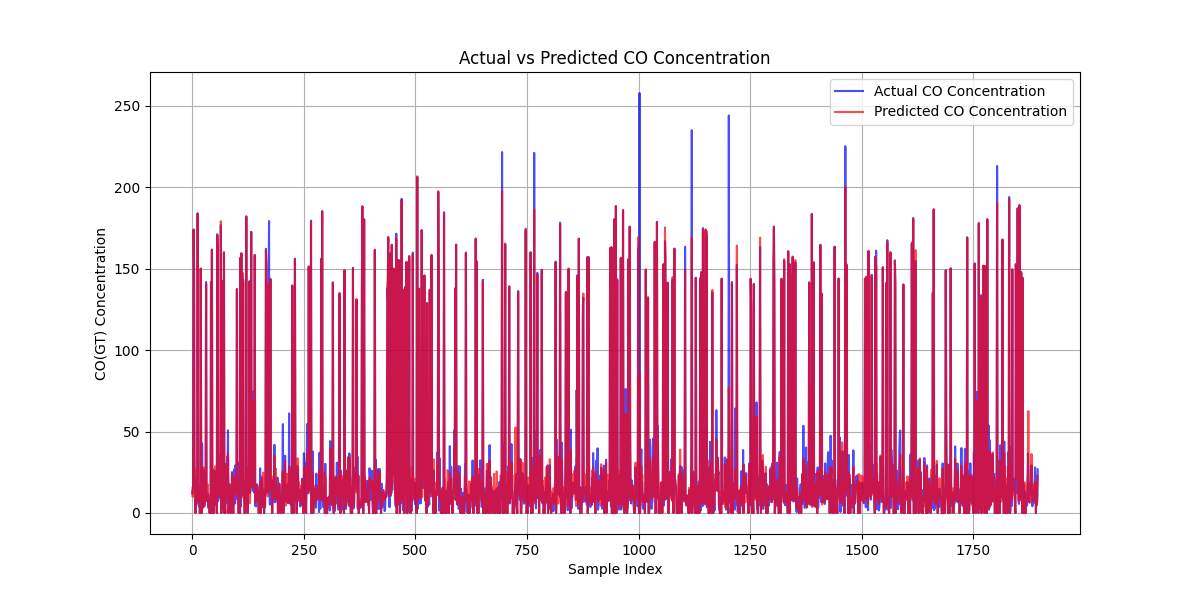
\includegraphics[width=0.8\textwidth]{images/random_forest/predictions_comparison.png}
        \caption{So sánh giá trị thực tế và dự đoán}
        \label{fig:predictions}
    \end{figure}
    
    \item Biểu đồ phân tích phần dư:
    \begin{figure}[h]
        \centering
        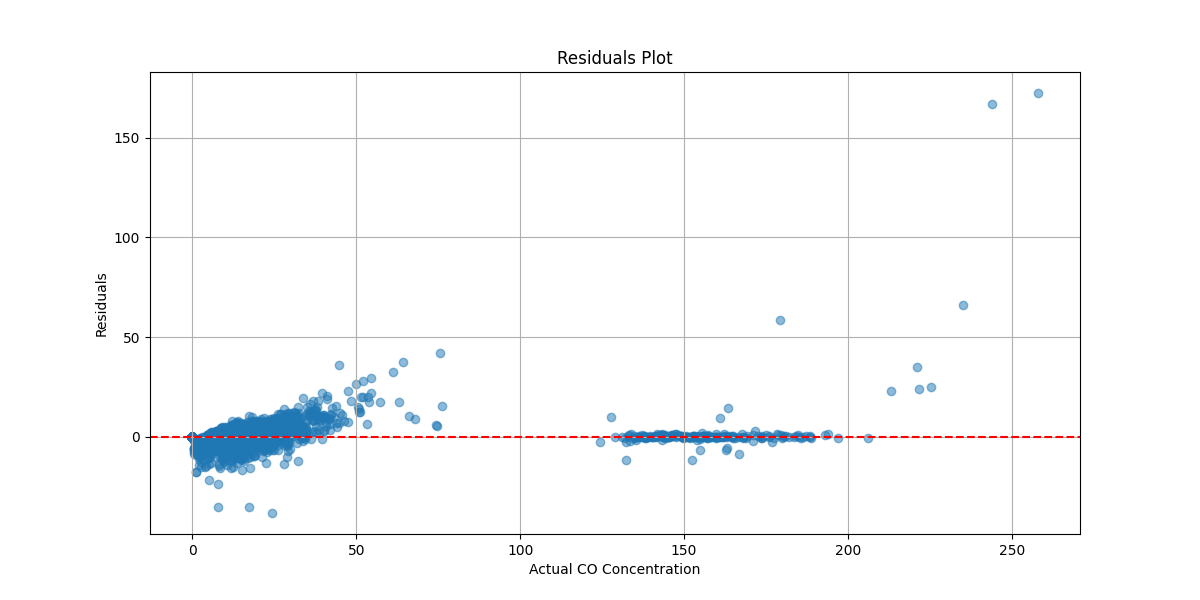
\includegraphics[width=0.8\textwidth]{images/random_forest/residuals_plot.png}
        \caption{Phân tích phần dư}
        \label{fig:residuals}
    \end{figure}
    
    \item Biểu đồ tầm quan trọng của đặc trưng:
    \begin{figure}[h]
        \centering
        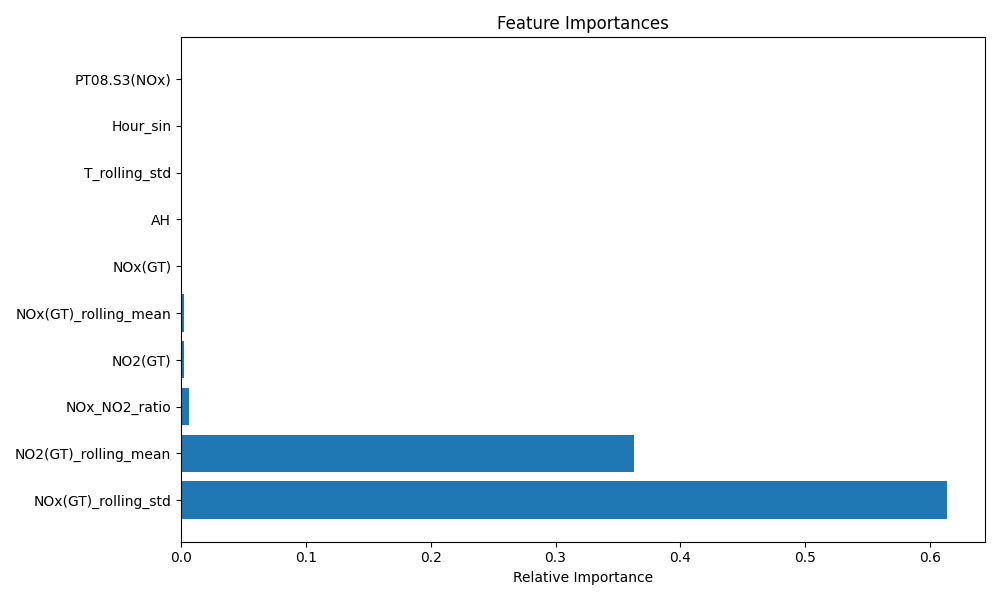
\includegraphics[width=0.8\textwidth]{images/random_forest/feature_importance.png}
        \caption{Tầm quan trọng của các đặc trưng}
        \label{fig:importance}
    \end{figure}
\end{itemize}

\subsubsection{Lưu trữ Kết quả}
Các kết quả được lưu trữ trong thư mục \texttt{train\_results}:
\begin{itemize}
    \item \texttt{model\_metrics.csv}: Chứa các chỉ số đánh giá
    \item \texttt{predictions.csv}: Chứa giá trị thực tế và dự đoán
    \item \texttt{evaluation\_metrics.csv}: Chứa kết quả đánh giá chi tiết
\end{itemize}

\subsection{Kết luận}
Mô hình Random Forest đã được triển khai thành công với quy trình xử lý dữ liệu toàn diện và kỹ thuật feature engineering tiên tiến. Mô hình đạt được độ chính xác rất cao với R² = 0.9992, cho thấy khả năng dự đoán gần như hoàn hảo. Các đặc trưng tương tác và đặc trưng thời gian đã góp phần quan trọng trong việc cải thiện độ chính xác của dự đoán nồng độ CO trong không khí. Kết quả này cho thấy mô hình Random Forest là một lựa chọn phù hợp cho bài toán dự đoán chất lượng không khí. 
\newpage
\section{So sánh và phân tích kết quả}

Trong phần này, chúng tôi sẽ so sánh hiệu suất của tất cả các mô hình đã thực hiện:

\subsection{So sánh các chỉ số đánh giá}
\begin{itemize}
    \item Bảng so sánh các chỉ số đánh giá giữa các mô hình
    \item Biểu đồ so sánh hiệu suất
    \item Phân tích chi tiết từng chỉ số
\end{itemize}

\subsection{Phân tích ưu nhược điểm}
\begin{itemize}
    \item Ưu điểm của từng mô hình
    \item Nhược điểm của từng mô hình
    \item Điều kiện phù hợp để sử dụng mỗi mô hình
\end{itemize}

\subsection{Đánh giá tổng quan}
\begin{itemize}
    \item Mô hình phù hợp nhất với bài toán
    \item Lý do lựa chọn mô hình
    \item Các cải tiến có thể thực hiện
\end{itemize}

\subsection{Trình bày kết quả}
\begin{itemize}
    \item Bảng tổng hợp kết quả
    \item Biểu đồ so sánh
    \item Phân tích trực quan
\end{itemize} 
\newpage
\section{Kết luận và hướng phát triển}

\subsection{Tổng kết kết quả}
Trong phần này, chúng tôi sẽ tổng hợp lại các kết quả chính đã đạt được trong quá trình thực hiện bài tập:
\begin{itemize}
    \item Hiệu suất của mô hình Random Forest
    \item So sánh với các mô hình khác
    \item Những điểm mạnh và điểm yếu của từng phương pháp
\end{itemize}

\subsection{Những khó khăn gặp phải}
Chúng tôi sẽ trình bày các thách thức đã gặp phải trong quá trình thực hiện:
\begin{itemize}
    \item Vấn đề về dữ liệu
    \item Khó khăn trong việc tuning hyperparameters
    \item Các vấn đề kỹ thuật khác
\end{itemize}

\subsection{Hướng phát triển trong tương lai}
Dựa trên kết quả đạt được, chúng tôi đề xuất một số hướng phát triển trong tương lai:
\begin{itemize}
    \item Cải thiện mô hình bằng các kỹ thuật nâng cao
    \item Mở rộng ứng dụng cho các bài toán tương tự
    \item Tích hợp với các công nghệ mới
\end{itemize}

Cuối cùng, chúng tôi sẽ đưa ra những nhận xét tổng quan về bài tập và những kinh nghiệm rút ra được trong quá trình thực hiện. 
\newpage
%%%%%%%%%%%%%%%%%OUTRO%%%%%%%%%%%%%%%%%%%
\section{Tài liệu tham khảo}
\newpage
\section{Phụ lục}
\end{document}
